\documentclass[10pt]{book}

% --- KDP 6x9 WITH BLEED: page = 6.125" x 9.25" ---
\usepackage[
paperwidth=6.125in,
paperheight=9.25in,
margin=0in
]{geometry}

% --- Packages ---
\usepackage[pages=all]{background}
\usepackage{graphicx}
\usepackage{tikz}
\usetikzlibrary{calc}
\usepackage{xcolor}
\usepackage{anyfontsize}
\usepackage[protrusion=true,expansion=true]{microtype}

\pagestyle{empty}
\setlength{\parindent}{0pt}

% --- Colors ---
\definecolor{coveraccent}{HTML}{00B7C2} % accent color
\definecolor{covertext}{HTML}{E6E6E6}   % light body text

% --- Background image ---
% Ideal: 300 dpi at 6.125"x9.25" approx. 1838 x 2775 px
% The file must be in the same folder as this .tex file.
\backgroundsetup{
	scale=1,
	angle=0,
	opacity=1,
	contents={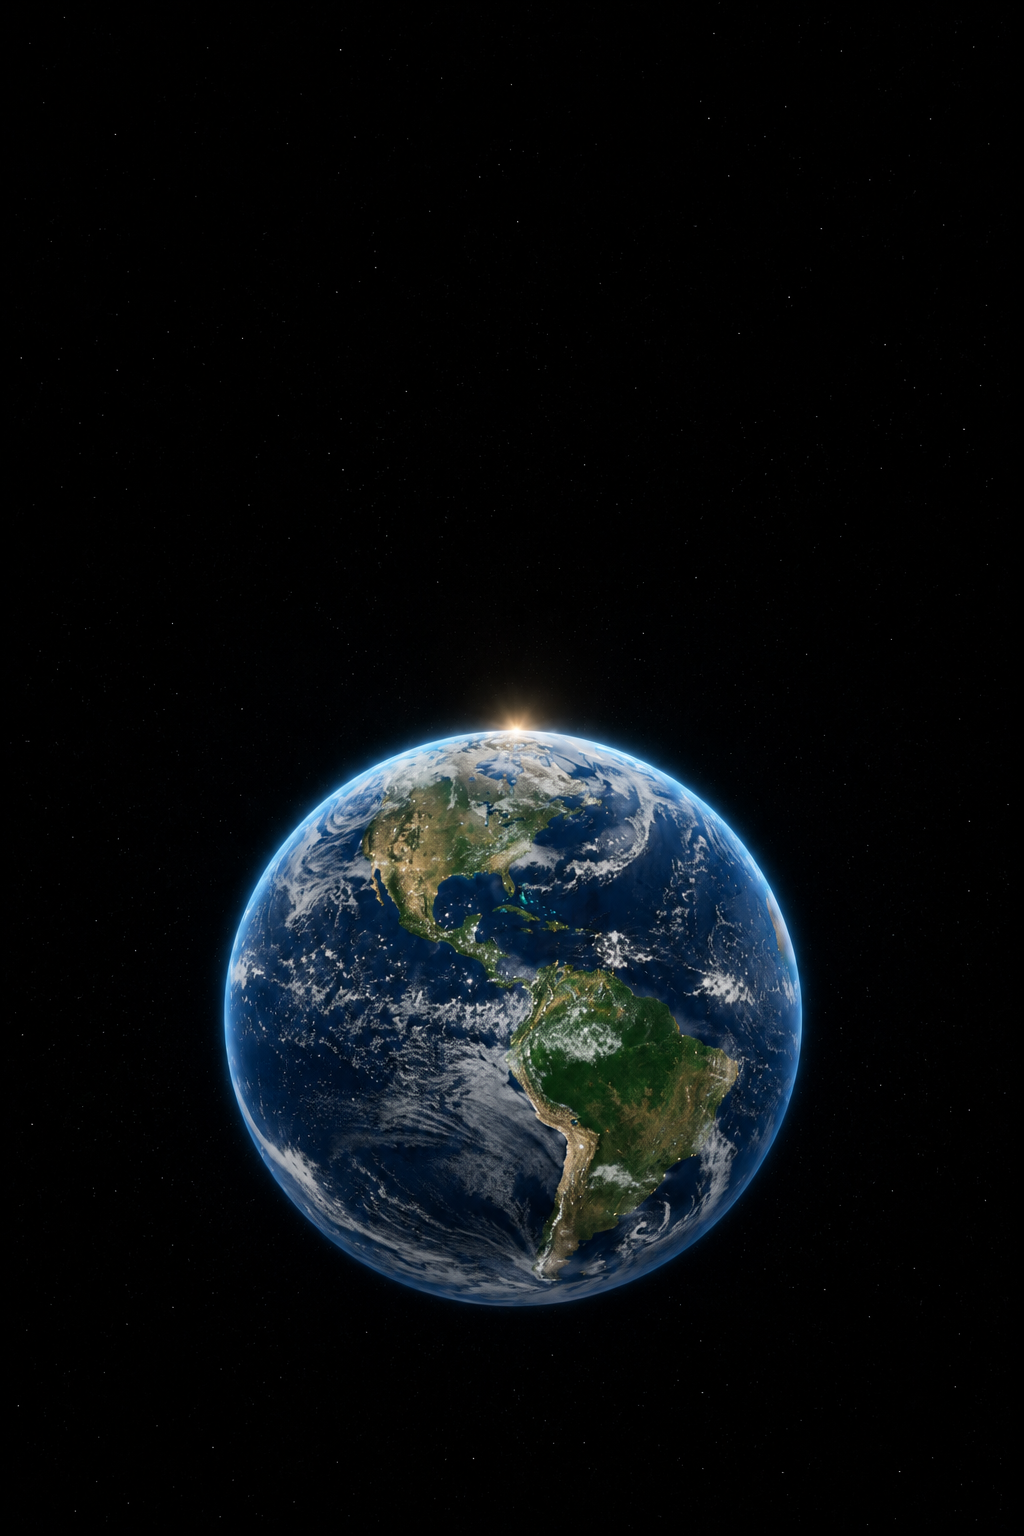
\includegraphics[width=\paperwidth,height=\paperheight]{03.png}}
}

% --- Safe-area offsets ---
\newlength{\bleed}\setlength{\bleed}{0.125in}
\newlength{\safe}\setlength{\safe}{0.35in}
\newlength{\inset}\setlength{\inset}{\dimexpr\bleed+\safe\relax} % = 0.475in

\begin{document}
	\thispagestyle{empty}
	
	% -------------------------------------------------
	% Back-cover text, absolutely positioned
	% -------------------------------------------------
	
\begin{tikzpicture}[remember picture,overlay]
		\node[
		anchor=north west,
		inner sep=0pt,
		text width=4.25in,
		align=justify
		] at ([xshift=1.0in,yshift=-.60in]current page.north west) {%
			
			% Title
			{\color{coveraccent}\fontsize{17}{21}\selectfont\bfseries\sffamily
				The Structure of the World\par}
			
			\vspace{0.45em}
			
			% Body text
			{\color{covertext}
				\fontsize{11.2}{15.0}\selectfont
				\sffamily
				\spaceskip=0.38em plus 0.16em minus 0.08em
				
				Is mathematics merely a human tool -- or does it describe a deeper order of reality?
				This book leads from numbers, geometry, natural laws, probability, and modern physics
				to the question of why the world is mathematically understandable at all.
				
				\medskip
				
				Mathematics appears here not as mere calculation, but as a universal structure:
				visible in forms, motion, symmetries, natural laws, and the limits of human thought.
				
				\medskip
				
				\textbf{For curious readers who do not merely want to apply mathematics, but truly understand it.}
				
				\medskip
				
				\emph{Christian Weilharter, Dipl.-Ing.(FH),} combines engineering thinking,
				mathematical curiosity, and a physical perspective.
				This book builds a bridge between clear explanation,
				scientific depth, and philosophical reflection.
			}
		};
	\end{tikzpicture}
	
\end{document}